The goal of this Chapter is to show how \name can improve the traditional top-down analysis method. Usually, researchers start from a deep comprehension of the theoretical problem  to to draw a model of the system over which is possible to formulate hypothesis. Further knowledge about  the implementation experience may support this method, however this approach is traditionally top-down. In this chapter we present an evaluation of \name Baselines (See Chapter \ref{sec:baselines}) in order to demonstrate how \name can extend the traditional hypothesis-based research towards the Systematic Comparative Research approach we introduced in Chapter \ref{chap:problem-settings}. Firstly, in section \ref{sec:experimental-setting} we describe the Experimental Setting, presenting our assumptions and two experiment sets for baselines evaluation. With the SOAK Test, in Section \ref{sec:soak-es}, we follow the traditional research method, showing its limitations with empirical results. In Section \ref{sec:step-es} we extends the research work on the baselines as an example of \name potential.

When the subject of our research are complex system, it is hard to formulate and prove hypothesis that are only based on he knowledge of the model. Indeed in Section \ref{sec:empirical-research} shows there is a lack in Computer Science about system evaluation. In this Chapter we present results of two kind of test, SOAK Tests and a case of stress test which study the step response of the system (see Section \ref{sec:software-testing}). The aim of SOAK tests is to show the problem dimension of traditional top-down analysis over complex software system, even for simple hypothesis, and consequently demonstrate that we need \namens . On the other hand, Step-Response test are designed to show \name potential.


\section{Experimental Setting}
\label{sec:experimental-setting}
The experimental setting is the set of rules, assumption and conventions the researchers specify before starting with the evaluation, i.e. the execution of experiment and the interpretation of the results. The experimental setting for our evaluation consists into the definition of different tests to cover the most important variations on the tuple that describes an experiment and briefly consist in (see Chapter \ref{chap:heaven} for further details): $<\mathcal{D}, \mathcal{T},\mathcal{E}, \mathcal{Q}>$, where:
\begin{itemize}
\item $\mathcal{E}$ is the RSP Engine
\item $\mathcal{D}$ is the Dataset 
\item $\mathcal{T}$ is the Ontology
\item $\mathcal{Q}$ is the Query that $\mathcal{E}$ continuously answers.
\end{itemize}


As we said in the introduction Top-Down investigations are commonly hard, and they are even harder for commercial solutions. The e architecture complexity of commercial solutions like C-SPARQL Engine and CQELS is high, and can not be easily faced in order formulate hypothesis of comparison.
We develop (Section \ref{sec:baselines} and implement (Section \ref{sec:baselines-impl}) the Baselines as the RSP Engines $\mathcal{E}$ subject of our experiment, in order to simplify the research survey and make it possible. Indeed, we have a complete model of the baseline systems and we also know many implementation details that can help during the analysis. Moreover, in Chapter \ref{chap:problem-settings} we describe which requirements guarantee that an RSP Engine is a baselines: Simplicity, Elementarily, Relevance and Eligibility (SERE properties) allow us to evaluate the baselines as a simple term of comparison for further research on Stream Reasoning systems and clarify how to develop the investigation.
 
The four baselines differ for two characteristics: RDF Stream Model and Reasoning architecture. The Table \ref{tab:baselines-names} summarises these few but well determined differences, naming the four baselines for the evaluation:\begin{table}[htb]
\scriptsize
\centering
\begin{tabular}{c|cc} % creating eight columns
	\hline
         & Naive & Incremental\\
	\hline
	Graph        &  B1      & B2\\
	Statment   &  B3   & B4\\
	\hline % inserts single-
\end{tabular}
\caption{Configuration of the four baselines, further details in Section \ref{sec:baselines}}
\label{tab:baselines-names}
\end{table}

\noindent Among these four configurations we formulate simple hypothesis, stating which approach is better then an other one within an experiment. Notice that we can exploit the know-how about their internal mechanisms, described in Section \ref{sec:baselines-impl}, to help to find the motivations behind behaviours which are unpredictable form the architectural viewpoint. 

The Dataset  $\mathcal{D}$ and the Ontology $\mathcal{T}$ must be chose to ensure baselines Simplicity, as stated in Section \ref{sec:baselines}. We take $\rho$DF  \cite{DBLP:conf/esws/MunozPG07} as their entailment regime, because several works in the field \cite{DBLP:conf/semweb/UrbaniMJHB13} choose this as the minimal meaningful task for a Stream Reasoner. In particular, $\rho$DF is the RDF-S fragment that reduce complexity while preserving the normative semantics and core functionalities. 

The RDF streams  $\mathcal{D}$ used in the experiments are obtained streaming in different ways the data generated with LUBM  \cite{Guo2005} and the ontology $\mathcal{T}$ is the LUBM one\footnote{http://swat.cse.lehigh.edu/onto/univ-bench.owl}. We assume that the ontology does not change over time, therefore the materialisation of $\mathcal{T}$ is computed before starting the experiment and the RSP engine does not have to perform this task. It is worth to discuss the choice of using data from LUBM (Section \ref{sec:lubm}) over SRbench (Section \ref{sec:srbench}) and LSbench(Section \ref{sec:ls:bench}). The first one has data, which are not adequate for the experiments, since they do not require any reasoning. The SRbench data, on the contrary, requires reasoning, but, being real-data, do not have the possibility to be scaled up and down. This choice is in line with previous works on Stream Reasoning \cite{DBLP:conf/semweb/UrbaniMJHB13}. 

The data generator system, responsible to build $\mathcal{D}$ w.r.t. $\mathcal{T}$, is able to scale both in terms of dimension of the dataset and the reasoning effort. Being LUBM static data, we exploit the \textit{RDF2RDFStream} component of the test stand that takes care to adapt the data generate by LUBM to a streaming scenario. The component can be set up to obtain an RDFStream where the number of triples with the same timestamps follows a given discrete function, Section \ref{sec:streamer-impl} contains all the details about the implementation and the usage of this particular \textsc{Streamer}. %e' veramente il timestamp quello?

We designed two kind of experiments based on the \textit{RDF2RDFStream} capabilities to control the triple distribution in the RDFStream. In order to evidence system dynamics over a particular input the first experiment typology belongs to the category of SOAK Test. The aim of the experiments in this Section is also to show what kind of testing is possible trough \namens, the second kind of experiment belongs to the category of Stress Test (Section \ref{sec:software-testing} describes the different kinds of software testing). In summary:

\begin{itemize}
\item \textbf{SOAK}: the number of contemporary triple in the RDFStream does not change during the experiment.
\item \textbf{Step Response} the number of contemporary triple suddenly changes during the experiment, usually increasing of a degree of magnitude.
\end{itemize}
 
The last parameter in the experiment tuple is the query $\mathcal{Q}$. Out  experiments uses variants of the same two basic identity queries that continuously asks for the materialisation of the current window:
\begin{enumerate}
\item[Q.1] Naive
\item[Q.2] Incremental
\end{enumerate}
 		 
Q.1 outputs the snapshot of the entire window and it is used for the Naive reasoning approach; Q.2 outputs the ir-streams and it is used for the Incremental reasoning approach. The queries differ for the size $\omega$ of the sliding window. In particular, we use windows in which $\omega$ is an integer multiple of the slide parameter $\beta$ of the window, i.e., it holds that $\omega = \beta * N$. In other words, $N$ is the number of \textsc{CTEvents} that the window contain. 

Moreover, Section \ref{sec:baselines-impl} shows how the proposed baselines take advantage of the ability of Esper to be temporally controlled by an external agent\footnote{\url{http://esper.sourceforge.net/esper-0.7.5/doc/reference/en/html_single/index.html#api-controlling-time}} by sending time-keeping events to synchronise the internal time flow. All the triples in the \textit{CTEvent} are consider contemporary by the baselines and each \textit{CTEvent} can be seen as a proxy for the timing event. Together with the \textit{RDF2RDFStream} is possible to estimate the content of the current window in terms of number of RDF Triples in any moment of the experiment.

We describe in details the content of the SOAK (Section \ref{sec:soak-es}) and the Step Response tests (Section \ref{sec:step-es}), providing a lecture key for the experiment results.

\section{Experiment Design}

Experiment design (ED) means project our experiment in order to prove or refute one or more hypothesis, evidencing the behaviour of the system in the context that those hypothesis involves. ED starts with some assumptions, we formulate ours in Section \ref{sec:experimental-setting} under Experimental Setting definition. In section above we explain, for example, the reasons why we chose $\rho$DF as entailment regime for our experiments. Researchers formulate hypothesis on the base of these assumption, Figure \ref{fig:experiment-design} summarises the collocation of ED within the Top-down approach.

\begin{figure}[tbh]
  \centering
	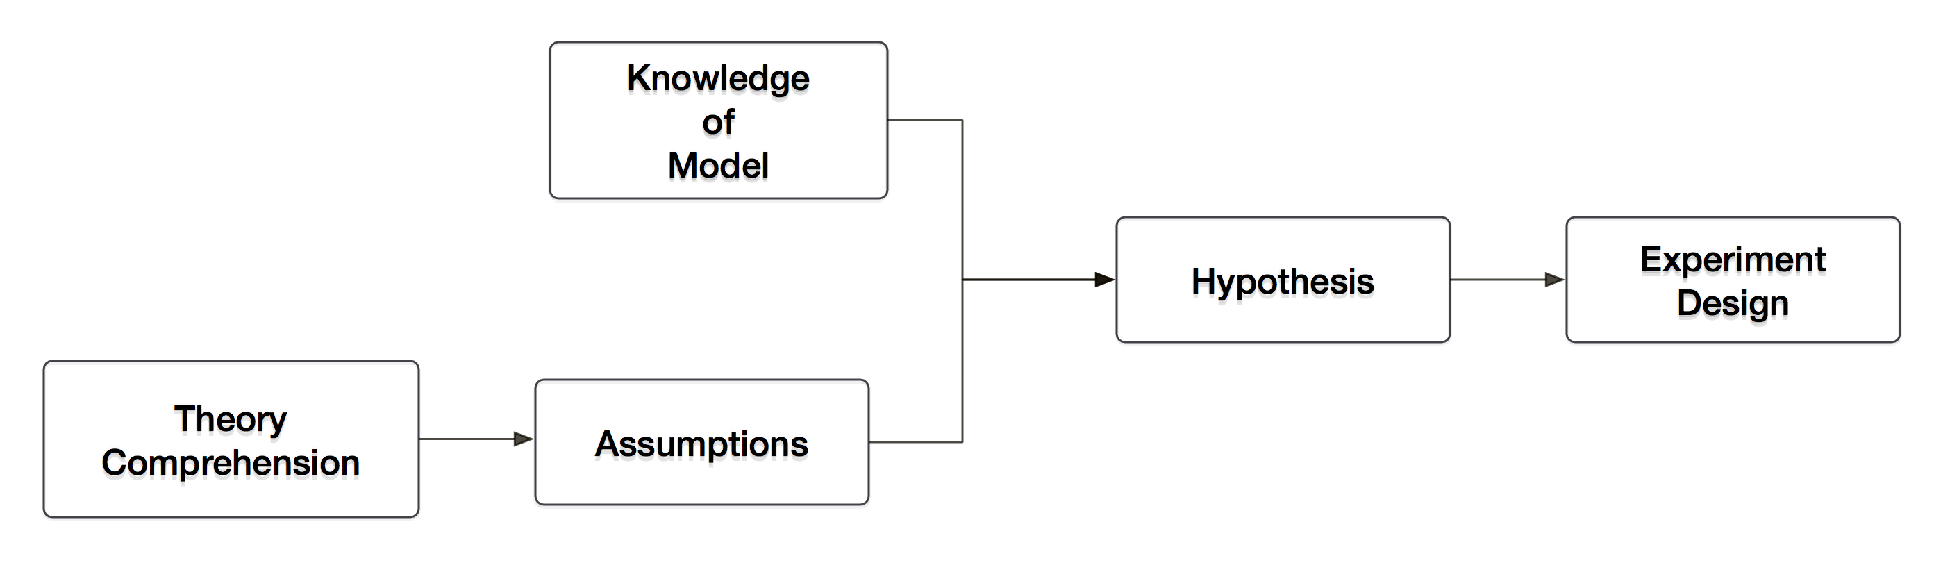
\includegraphics[width=\linewidth]{images/experiment-design}
	\caption{Traditional Experiment design workflow} 
  	\label{fig:experiment-design}
\end{figure}


From a theoretical point of view we decide to study RSP Engine facing their nature of linear dynamic system.(see Section \ref{sec:sfp}). Experiment design requires to point out which variable are observed. We simplify the study analysing their behaviour in term of Latency and Memory, which is the minimal meaningful measurement set for an RSP Engine (Chapter \ref{chap:heaven}). Finally we compare the results of the four baselines (see Table \ref{tab:baselines-names}) between many experiments.

\subsection{SOAK: Tests and Hypothesis}\label{sec:soak-es}

Soak testing show the system dynamics, stressing the subject with a constant and continuous input flow. In the Stream Reasoning context the RDFStream is controlled to have the same number of contemporary triple over time. 

All the experiments are 20000 events long, this duration ensures to reach for majority of the experiments the Steady State condition for both latency and the memory. Unlikely, is not possible to foretell how many events are required in to reach the Steady State condition for a certain variable, especially memory. Multiple attempts and empirical evaluation are the only way to set up the correct longness. All experiment are executed 10 times, and we take the average to reduce measurement error. 

\begin{table}[htb]
\centering
 \begin{tabular}{l|c| lllll}
	  	\hline
		\multicolumn{2}{c|}{  } &\multicolumn{5}{c}{Window size}  \\
		\multicolumn{2}{c|}{  } & 1 & 10 & 100 &1000 &10000\\
		\hline
		\hline
		 & 1 & 1 & 10 & 100 & 1000&10000 \\
		\textsc{CTEvent}      & 10  & 10  & 100  & 1000 & 10000  \\
		size             &100   & 100   & 1000 & 10000  \\
					&1000   & 1000 & 10000 \\
					&10000   & 10000  \\
		\hline 
	\end{tabular}
	
	 \vspace{10pt}
	\caption{The number of triples in the window during the ten SOAK tests as a function of the Window size (in terms of $N$) and of the triples in each \textsc{CTEvent}.}
	\label{tab:soaktests}
\end{table}

Table \ref{tab:soaktests} presents the fifteen SOAK tests we run for each baseline presented in Table \ref{tab:baselines-names}. The columns of the table are the different window sizes measured in terms of the values assumed by $N$.  Being $\beta=$ 100 ms., they correspond to a window that spans 100 ms., 1 sec., 10 sec. and 100 sec.. The rows are the different number of triples in each \textit{CTEvent} sent by the \textsc{RDF2RDFStream} to $\mathcal{E}$. Notably, for all of them, we checked that $\mathcal{E}$ is responsive for the whole duration of the experiment. 

Following the traditional research method, we formulate two naive hypothesis based on the knowledge we have of the model. The hypothesis to verify with SOAK experiments are:
\begin{itemize}
\item \textbf{HP.1} The Incremental reasoning approach is always better then the naive one.
\item \textbf{HP.2} The Graph-based model for RDFStream is always better then the Triple-based one.
\end{itemize}

Notice that the goal of our research is to show how \name helps RSP Engine analysis trough empirical evaluations. Hypothesis verification and top-down analysis are the subject of our survey, while our research question is:  "\textit{Can an engine test stands, together with queries, datasets and methods, support Systematic Comparative Research Approach for Stream Reasoning?}" %"Needs the Stream Reasoning research field a Test Stand like \name to investigate RSP Engines and sustain the research of such system with an Systematic Comparative Approach?"

\subsection{Step Response Tests}\label{sec:step-es}

Step Response testing allow to see how the system reacts to a sudden changing in the input condition. They usually follow SOAK testing, which may show an initial warm-up phase for the systems. With this set of experiments we can study how the system response changes if we move form an input condition to another one from a stable running condition instead of starting from scratch.

We design the step experiments concatenating two of the SOAK table ones, obtaining a total length of 400000 events, which means hours of execution for the system. For this reason we investigate only few configuration, all with 10  window slot size for all the four baselines. Table \ref{tab:steptests} summarises the step experiment set-up, where the step is positioned at the half of the execution, 20000 events.
\begin{table}[htb]
\centering
 \begin{tabular}{c|c|c}
	  	\hline
	  	&\multicolumn{2}{c}{CTEvent size}  \\
		Window Size & Initial Size & Final Size\\
		\hline
		\hline
		 10 & 10 & 100\\
		  10 & 100 & 1000\\
		 10 & 10 & 1000\\
		% 10 & 10 & 10000\\
		
		% 10 & 100 & 10000\\
		% 10 & 1000 & 10000\\
		\hline 
 \end{tabular}
	\vspace{10pt}
 \caption{}
\label{tab:steptests}
\end{table}

We do not formulate hypothesis for Step experiments. The purpose of this test set is to show \name capabilities and not to offers a deep understating of the baselines. However, we comment the results evidencing the finding in the sections below.

\subsection{Execution Environment}\label{sec:execution-environment}

All experiment are executed exploiting a dedicated machine, an iMac mid-2011 with 12GB RAM and 3.6 Ghz of a Intel i5 64 Bit, which run OS X 10.10.2 Yosemite,. Since \name is developed with Java 7\footnote{http://www.oracle.com/technetwork/java/javase/javase7locales-334809.html}, we use the versione 1.7.0.71 of the JVM.
The execution happens in a controlled environment, which tries to reduce the number of disturbing elements like network, graphical interface and other running processes.

\section{Evaluation Results}



Section \ref{sec:analyser-impl} shows the different level of analysis powered by \namens. We start presenting the SOAK Results exploiting the high level dashboard view: Figure \ref{fig:result_dashboard} shows how the baselines behaviour changes while changes the experimental setting. We compare the variation of the slot number in the active window, starting from 1 (tumbling) and moving to 10000, Figure \ref{fig:results_diagonal_5} shows this comparison.
What results state is that not only both the Hypothesis we have formulated in Section \ref{sec:soak-es} are not confirmed for all the experiment, but also that there is not a baseline which wins all the contrasts. This evidence states how difficult is to prove theoretical truth in complex system like RSP Engines, even for the Baselines which are simpler than the commercial solutions.

\name allows to better understand these results going deeply in the analysis. First of all we present in Tables \ref{tab:soak_latency_comparisons} and \ref{tab:soak_memory_comparisons}, which resumes in all the experiment which Baselines i better, fixing a certain property. Here we include the symbolic resuming table, but \name allow visualisation also of the numerical result, for a direct analysis

Tables \ref{tab:soak_latency_comparisons}  and \ref{tab:soak_memory_comparisons} show in a easy-to-read form the behaviour in terms of latency and memory. Some observation are possible on this data, because \name changes the way to investigate RSP Engines: now we can state some empirical truths and we can improve our models. 

The results in Table \ref{tab:soak_latency_comparisons}.c and Table \ref{tab:soak_latency_comparisons}.d when N=1, i.e., the window contains only one \textit{CTEvent},  allow to state for large events that the Naive approach is faster than the Incremental one. Instead, when \textit{CTEvent} contains only few triples, the Incremental approach is faster. This is not intuitive, because from theory we know that the incremental maintenance is more computationally expensive then materialisation for large changes \cite{DellAglio2014,DBLP:conf/cikm/RenP11,DBLP:conf/semweb/UrbaniMJHB13}.

When $N>$1, the results in Table \ref{tab:soak_latency_comparisons}.a and \ref{tab:soak_latency_comparisons}.b allow to say that using a Triple-base RDF stream is faster than Graph-based one. This is because the graph data structure may speed up reasoning when it contains multiple triple, but it does so introducing an overhead that may hinder performances when it contains few triples \cite{DBLP:conf/semweb/BalduiniVDTPC13}.   In particular, for the case $N$=1000 when the window contains 1000 triples (i.e., each \textsc{CTEvent} contains only one triple),  the Naive Triple-based approach is about 10\% faster  than the Naive Graph-based one while the Incremental Graph-based is even about 20\% faster.

Finally, the results in Table \ref{tab:soak_latency_comparisons}.c and \ref{tab:soak_latency_comparisons}.d supports the idea that when the number of changing triples in $\Delta+ \Delta-$ (Section \ref{sec:baselines}) is a small fraction of those in the window an Incremental approach is faster than the Naive one \cite{DellAglio2014,DBLP:conf/cikm/RenP11,DBLP:conf/semweb/UrbaniMJHB13}. The exception of the case $N$=1, but it can be considera limit case, where the reasoner is asked to deduce all the implicit triples implied by the only explicit triple in the window.  

While is possible to state meaningful observation over latency data, the same is not possible for memory ones. \name shows that the study of the memory can not be faced with the same methods to study latency, comparing the mean values at the Steady State condition. Table \ref{tab:soak_memory_comparisons} reports the  results for the memory usage during the experiments with the same representation we used for latency.  It is very hard to identify common behaviour in those results, and we can't confirm the what we observed in Table \ref{tab:soak_latency_comparisons}. However, trough \name is possible to lead the analysis to another level, observing the directly the memory usage in the time domain or in the frequency domain. 


\pagebreak
\begin{table}[htbp]
	\centering
	
	\subtable[Incremental]{%
		\begin{tabular}{l | ccccc} % creating eight columns
	  	\hline
		Triple in & \multicolumn{5}{c}{Number of Slots}  \\
		 Window  & 1 & 10 & 100 & 1000&10000 \\
		\hline
		1  	 & $\simeq$\\
		10   & Graph     &  	$\simeq$  \\
		100  & Graph     & 	$\simeq$  & $\simeq$\\
		1000 & Graph     & 	$\simeq$  & Triple & Triple\\
		10000 & Graph     & Triple  & Triple & Triple&Triple\\
		\hline % inserts single-line
	 \end{tabular}
	}\qquad\qquad
	\subtable[Naive]{%
		\begin{tabular}{l | ccccc} % creating eight columns
	  	\hline
		Triple in & \multicolumn{5}{c}{Number of Slots}  \\
		 Window  & 1 & 10 & 100 & 1000&10000 \\
		\hline
		1  	 & Graph\\
		10   & Graph     &  	Triple  \\
		100  & Graph     & 	Triple  & Triple\\
		1000 & Graph     & 	Triple  & Triple & Triple\\
		10000 &  Triple    & 	$\simeq$  & 	$\simeq$ & Triple&Triple\\
		\hline % inserts single-line
	 	\end{tabular}
	}\qquad\qquad
	\subtable[Graph]{%
		\begin{tabular}{l | ccccc} % creating eight columns
	  	\hline
		Triple in & \multicolumn{5}{c}{Number of Slots}  \\
		 Window  & 1 & 10 & 100 & 1000&10000 \\
		\hline
		1    & INC\\
		10   & INC   & INC \\
		100  & NAIVE & INC & INC\\
		1000 & NAIVE & INC & INC & INC\\
		10000 & NAIVE & INC & INC & INC& INC\\
		\hline % inserts single-line
		\end{tabular}
	}\qquad\qquad
	\subtable[Triple]{%
		\begin{tabular}{l | ccccc} % creating eight columns
	  	\hline
		Triple in & \multicolumn{5}{c}{Number of Slots}  \\
		 Window  & 1 & 10 & 100 & 1000&10000 \\
		\hline
		1    & INC\\
		10   & INC   & INC \\
		100  & NAIVE & INC & INC\\
		1000 & NAIVE & INC & INC & INC\\
		10000 & NAIVE & INC & INC & INC& INC\\
		\hline % inserts single-line
		\end{tabular}
	}	
	\caption{(a), (b) - latency results comparison between Incremental and Naive approaches; (d), (c) - results comparison between Graph-based and Triple-based models}
	\label{tab:soak_latency_comparisons}	
\end{table}
\pagebreak

\pagebreak
\begin{table}[htbp]
	\centering
	
	\subtable[Incremental]{%
		\begin{tabular}{l | ccccc} % creating eight columns
	  	\hline
		Triple in & \multicolumn{5}{c}{Number of Slots}  \\
		 Window  & 1 & 10 & 100 & 1000&10000 \\
		\hline
		1  	 & $\simeq$\\
		10   & Graph     &  	$\simeq$  \\
		100  & Triple     & 	Triple & Triple\\
		1000 & Graph     & 	Triple  & $\simeq$ & Triple\\
		10000 & $\simeq$     & Graph  & $\simeq$ & Triple&Graph\\
		\hline % inserts single-line
	 \end{tabular}
	}\qquad\qquad
	\subtable[Naive]{%
		\begin{tabular}{l | ccccc} % creating eight columns
	  	\hline
		Triple in & \multicolumn{5}{c}{Number of Slots}  \\
		 Window  & 1 & 10 & 100 & 1000&10000 \\
		\hline
		1  	 & Graph\\
		10   & Graph     &  	Graph  \\
		100  & Triple     & 	Graph  & Graph\\
		1000 & Graph     & 	Triple  & Triple & Graph\\
		10000 &  $\simeq$    & 	Graph & 	Graph & $\simeq$&Triple\\
		\hline % inserts single-line
	 	\end{tabular}
	}\qquad\qquad
	\subtable[Graph]{%
		\begin{tabular}{l | ccccc} % creating eight columns
	  	\hline
		Triple in & \multicolumn{5}{c}{Number of Slots}  \\
		 Window  & 1 & 10 & 100 & 1000&10000 \\
		\hline
		1    & INC\\
		10   & INC   & INC \\
		100  & INC & NAIVE	 & INC\\
		1000 & INC & NAIVE & NAIVE & NAIVE\\
		10000 & $\simeq$ & NAIVE & INC & INC& INC\\
		\hline % inserts single-line
		\end{tabular}
	}\qquad\qquad
	\subtable[Triple]{%
		\begin{tabular}{l | ccccc} % creating eight columns
	  	\hline
		Triple in & \multicolumn{5}{c}{Number of Slots}  \\
		 Window  & 1 & 10 & 100 & 1000&10000 \\
		\hline
		1    & INC\\
		10   & INC   & INC \\
		100  & INC & INC & INC\\
		1000 & NAIVE & NAIVE & NAIVE & NAIVE\\
		10000 & $\simeq$ &  $\simeq$ & INC & INC& NAIVE\\
		\hline % inserts single-line
		\end{tabular}
	}	
	\caption{(a), (b) - memory results comparison between Incremental and Naive approaches; (d), (c) - results comparison between Graph-based and Triple-based models}
	\label{tab:soak_memory_comparisons}	
\end{table}
\pagebreak



